\documentclass[10pt, aspectratio=43]{beamer}

% Carga la plantilla limpia personalizada
\usepackage{beamerthemecolmenar}

\title[Tecnología de Elementos]{MÉTODO DE LOS ELEMENTOS FINITOS}
\institute{Universidad Politécnica de Madrid}
\date{}

\begin{document}

% ==============================================================================
% PORTADA
% ==============================================================================
\begin{frame}
  \vfill
  \begin{uicard}[borderline north={4.5pt}{0pt}{DarkSlate}, left=16pt, right=16pt, top=22pt, bottom=22pt]
    \centering
    \vspace{0.2cm}
    {\large\bfseries \textcolor{Turquoise}{MÉTODO DE LOS ELEMENTOS FINITOS}}\\[0.7cm]
    
    {\Large \textcolor{DarkSlate}{\textbf{Tema 4: Tecnología de Elementos}}}\\[1.1cm]
    
    {\small \textcolor{TextDark!85}{\textbf{Escuela Técnica Superior de Ingenieros de Caminos, Canales y Puertos}}}\\[0.15cm]
    \textcolor{TextDark!65}{\footnotesize Universidad Politécnica de Madrid}
    \vspace{0.2cm}
  \end{uicard}
  \vfill
\end{frame}

% ==============================================================================
% ÍNDICE GENERAL
% ==============================================================================
\begin{frame}{Índice General}{Organización de la lección}
  \tableofcontents
\end{frame}

% ==============================================================================
% SECTION 1: BLOQUEO
% ==============================================================================
%%%%%%%%%%%%%%%%%%%%%%%%%%%%%%%%%%%%%%%%%%%%%%%%%%%%%%%%%%%%%%%%%%%%%%%%%%%%%%
\section[Bloqueo]{El fenómeno de bloqueo}
%%%%%%%%%%%%%%%%%%%%%%%%%%%%%%%%%%%%%%%%%%%%%%%%%%%%%%%%%%%%%%%%%%%%%%%%%%%%%%
\begin{frame}{El fenómeno de bloqueo}{Origen físico y matemático}
  \begin{uicard}[title=Restricciones físicas habituales]
    \begin{itemize}
      \item \textbf{Elasticidad incompresible ($\nu \to 0.5$):} Conservación estricta del volumen.
      \item \textbf{Flexión en elementos delgados ($t \to 0$):} Deformación por cortante nula (Kirchhoff-Love).
      \item \textbf{Plasticidad isocórica:} Deformaciones plásticas sin cambio de volumen.
    \end{itemize}
  \end{uicard}

  \vspace{0.1cm}

  \begin{uicard}[title=¿Por qué se produce el bloqueo?]
    El MEF busca el mínimo de la energía potencial en un espacio cinemáticamente restringido (polinomios a trozos). Al añadir restricciones físicas adicionados, el sistema queda \textbf{sobredeterminado} y la única solución admisible resulta ser la \textbf{solución nula} ($u \approx 0$).
  \end{uicard}
\end{frame}
%%%%%%%%%%%%%%%%%%%%%%%%%%%%%%%%%%%%%%%%%%%%%%%%%%%%%%%%%%%%%%%%%%%%%%%%%%%%%%
\begin{frame}
\frametitle{Elasticidad incompresible}
\begin{itemize}
\item Ecuación constitutiva (medio elástico isótropo):
$$
\sigma_{ij}=\lambda u_{k,k} \delta_{ij}+2 \mu u_{(i,j)}
$$

Si $\nu \rightarrow \frac{1}{2}$, entonces $\lambda=\frac{2 \nu \mu}{1-2\nu}
\rightarrow \infty$

La formulación en este caso será:
\begin{align*}
\sigma_{ij}&=-p \delta_{ij}+2 \mu u_{(i,j)} \\
u_{i,i}&=0
\end{align*}
\item Para triángulos lineales de presión constante, se tiene:
$$\int_{\Omega_e} \delta p^h u^h_{i,i} d\Omega=0 \;\; \forall \delta p^h \mbox{cte en
} \Omega_e
\Rightarrow \int_{\Omega_e} u^h_{i,i} d\Omega=0$$
es decir, los elementos no cambian de volumen:
\end{itemize}
\end{frame}
%%%%%%%%%%%%%%%%%%%%%%%%%%%%%%%%%%%%%%%%%%%%%%%%%%%%%%%%%%%%%%%%%%%%%%%%%%%%%%

\begin{frame}{Elasticidad incompresible}{Bloqueo en triángulos}
  \begin{columns}[c]
    \begin{column}{0.6\textwidth}
      \begin{center}
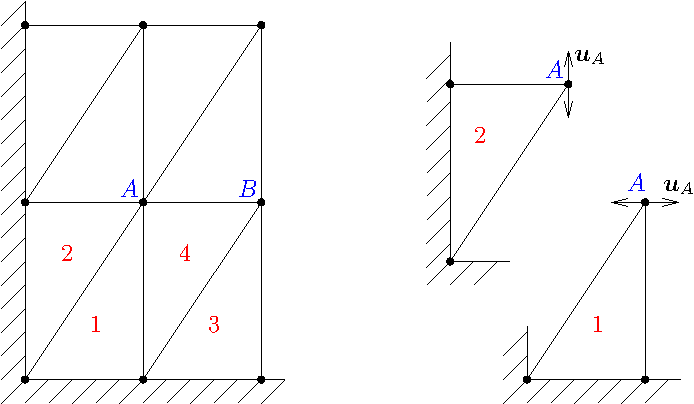
\includegraphics[width=0.95\textwidth]{bloqueo.pdf}
      \end{center}
    \end{column}

    \begin{column}{0.4\textwidth}
    {\footnotesize
      \begin{uicard}[title=Mecanismo de bloqueo]
        \begin{itemize}
          \item Para el triángulo $T1$, la incompresibilidad impone $\Delta V_e = \int_{\Omega_e} u_{i,i} \, d\Omega = 0$.
          \item Al fijar el contorno, imponer volumen constante elemento a elemento \textbf{congela los nodos internos} ($u_A = u_B = 0$).
          \item El sistema se vuelve infinitamente rígido.
        \end{itemize}
      \end{uicard}
      }
    \end{column}
  \end{columns}
\end{frame}
%%%%%%%%%%%%%%%%%%%%%%%%%%%%%%%%%%%%%%%%%%%%%%%%%%%%%%%%%%%%%%%%%%%%%%%%%%%%%%
\begin{frame}
\frametitle{Bloqueo y Elasticidad incompresible}
\begin{itemize}
\item Formulación válida para medios compresibles e incompresibles:
\begin{align*}
\sigma_{ij}&=-p \delta_{ij}+2 \mu u_{(i,j)} \\
u_{i,i}+\frac{p}{\lambda}&=0
\end{align*}
\item Observaciones
\begin{align*}
\nu&=\frac{1}{2} \Rightarrow p=-\frac{\sigma_{ii}}{3} \\
\nu &\approx \frac{1}{2} \Rightarrow p \approx -\frac{\sigma_{ii}}{3} \\
\nu &\neq \frac{1}{2} \Rightarrow p=-\lambda u_{i,i} \neq
\frac{\sigma_{ii}}{3}
\end{align*}
\end{itemize}
\end{frame}

% ==============================================================================
% SECTION 2: PATCH TEST
% ==============================================================================
\section[Patch test]{La prueba de la parcela y el análisis espectral (Q4)}

%%%%%%%%%%%%%%%%%%%%%%%%%%%%%%%%%%%%%%%%%%%%%%%%%%%%%%%%%%%%%%%%%%%%%%%%%%
\begin{frame}{La prueba de la parcela}{Condición de convergencia y diagnóstico}
{\footnotesize
  \begin{uicard}[title=Requisitos fundamentales del Patch Test]
    \begin{itemize}
      \item \textbf{Deformación constante:} Debe representar de forma exacta estados de tensión/deformación constante y movimientos de sólido rígido.
      \item \textbf{Verificación:} Ha de cumplirse para un solo elemento e incluso en \textbf{mallas distorsionadas}.
    \end{itemize}
  \end{uicard}

  \vspace{0.1cm}

  \begin{uicard}[title=Comportamiento de los modos de flexión]
    \begin{itemize}
      \item Todos los elementos válidos capturan el sólido rígido y la tensión constante. La diferencia entre formulaciones radica en la \textbf{rigidez de los modos de flexión}.
      \item \textbf{Bloqueo:} Aparece si la rigidez a flexión tiende a infinito ($\lambda_{\text{flex}} \to \infty$).
      \item \textbf{Hourglassing:} Aparece si la rigidez a flexión se anula ($\lambda_{\text{flex}} = 0$) por integración reducida.
    \end{itemize}
  \end{uicard}
  }
\end{frame}

%%%%%%%%%%%%%%%%%%%%%%%%%%%%%%%%%%%%%%%%%%%%%%%%%%%%%%%%%%%%%%%%%%%%%%%%%%
\begin{frame}
\frametitle{Modos de deformación}
\begin{itemize}
\item Para el elemento bilineal de $4$ nodos los modos de deformación son:

\vspace{5mm}
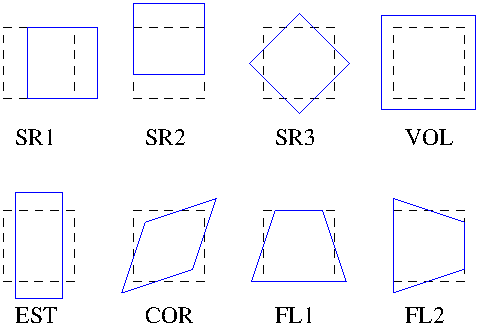
\includegraphics{modosq4}
\end{itemize}
\end{frame}
%%%%%%%%%%%%%%%%%%%%%%%%%%%%%%%%%%%%%%%%%%%%%%%%%%%%%%%%%%%%%%%%%%%%%%%%%%

\begin{frame}{Análisis espectral en Q4}{Autovalores de la matriz de rigidez $K^e$}
  % CARD 1: SÓLIDO RÍGIDO
  \begin{uicard}[title=Modos de sólido rígido, top=2pt, bottom=2pt, left=6pt, right=6pt, attach title to upper={\par\vspace{0.05cm}}]
    \small
    \centering
    $\lambda_{\text{SR1}} = \lambda_{\text{SR2}} = \lambda_{\text{SR3}} = 0$ \quad {\footnotesize (Autovalores nulos correctos)}
  \end{uicard}

  \vspace{0.05cm}

  % CARD 2: MODO VOLUMÉTRICO
  \begin{uicard}[title=Modo volumétrico, top=2pt, bottom=2pt, left=6pt, right=6pt, attach title to upper={\par\vspace{0.05cm}}]
    \footnotesize
    $$\lambda_{\text{VOL}} = \frac{1}{2r}\left[(\lambda+2\mu)(1+r^2) + \sqrt{4\mu(\lambda+\mu)(r^2-1)^2 + \lambda^2(r^2+1)^2}\right]$$
    \vspace{-0.1cm}
    \begin{center}
      \textbf{Diagnóstico:} En el límite incompresible ($\nu \to 0,5 \Rightarrow \lambda \to \infty$),\\
      \textcolor{YellowBC}{$\lambda_{\text{VOL}} \to \infty$} $\to$ \textbf{Bloqueo volumétrico}.
    \end{center}
  \end{uicard}

  \vspace{0.05cm}

  % CARD 3: MODOS DE FLEXIÓN
  \begin{uicard}[title=Modos de flexión \quad {\small($r = h/b$)}, top=2pt, bottom=2pt, left=6pt, right=6pt, attach title to upper={\par\vspace{0.05cm}}]
    \footnotesize
    $$\lambda_{\text{BG1}} = \frac{\mu + (\lambda+2\mu)r^2}{3r}, \qquad \lambda_{\text{BG2}} = \frac{\mu r^2 + \lambda + 2\mu}{3r}$$
    \vspace{-0.1cm}
    \begin{center}
      \textbf{Diagnóstico:} En esbeltez ($r \to \infty$) o incompresibilidad ($\lambda \to \infty$),\\
      \textcolor{YellowBC}{$\lambda_{\text{BG}} \to \infty$} $\to$ \textbf{Bloqueo en flexión}.
    \end{center}
  \end{uicard}
\end{frame}

%%%%%%%%%%%%%%%%%%%%%%%%%%%%%%%%%%%%%%%%%%%%%%%%%%%%%%%%%%%%%%%%%%%%%%%%%%
\begin{frame}
\frametitle{Conclusiones}
  \begin{uicard}[title=Causa fundamental del problema, top=3pt, bottom=4pt, left=8pt, right=8pt, attach title to upper={\par\vspace{0.08cm}}]
    \small
    \begin{itemize}
      \item Surge por una \textbf{excesiva rigidez numérica} al imponer restricciones físicas sobre espacios de interpolación pobres (como la interpolación lineal de deformaciones volumétricas y de corte).
      \item El sistema resulta \textbf{sobredeterminado}, forzando desplazamientos casi nulos ($u \approx 0$).
    \end{itemize}
  \end{uicard}

  \vspace{0.15cm}

  \begin{uicard}[title=Estrategia de resolución, top=3pt, bottom=4pt, left=8pt, right=8pt, attach title to upper={\par\vspace{0.08cm}}]
    \small
    \begin{itemize}
      \item Es necesario \textbf{modificar la formulación} en los términos asociados a las deformaciones no constantes.
      \item La \textbf{integración reducida} elimina el bloqueo al simplificar dicho campo, pero introduce un nuevo riesgo: la aparición de \textbf{modos espúreos de energía nula} (\emph{hourglassing}).
    \end{itemize}
  \end{uicard}
\end{frame}
%%%%%%%%%%%%%%%%%%%%%%%%%%%%%%%%%%%%%%%%%%%%%%%%%%%%%%%%%%%%%%%%%%%%%%%%%%
\begin{frame}
\frametitle{Tecnologías especiales}
\begin{enumerate}
\item Métodos mixtos.
\item Integración selectiva y reducida.
\item Control de Hourglass
\item Formulación $\overline{\bm{B}}$
\item El método de los modos incompatibles
\item Formulación con deformaciones supuestas mejoradas
\end{enumerate}
\end{frame}

 
% ==============================================================================
% SECTION 3: Formulación Mixta
% ==============================================================================

%%%%%%%%%%%%%%%%%%%%%%%%%%%%%%%%%%%%%%%%%%%%%%%%%%%%%%%%%%%%%%%%%%%%%%%%%%
\section[Formulación Mixta]{Formulaciones mixtas}
%%%%%%%%%%%%%%%%%%%%%%%%%%%%%%%%%%%%%%%%%%%%%%%%%%%%%%%%%%%%%%%%%%%%%%%%%%
\begin{frame}
\frametitle{Introducción}
\begin{itemize}
\item Las referencias son muy abundantes
\item Los métodos mixtos emplean diferentes interpolaciones para diferentes
campos: desplazamientos-presión, desplazamientos-tensión,
desplazamientos-deformación, etc.
\item Para que una formulación mixta tenga garantizada la convergencia, ha de
verificar la condición de Babuska-Brezzi (problema de checker-board).
\item Los elementos de orden alto pierden robustez en problemas no lineales.
\item No hay un ``buen elemento'' para todas las clases de problemas
\end{itemize}
\end{frame}
%%%%%%%%%%%%%%%%%%%%%%%%%%%%%%%%%%%%%%%%%%%%%%%%%%%%%%%%%%%%%%%%%%%%%%%%%%
\begin{frame}
\frametitle{Formulación fuerte}
\begin{itemize}
\item Dados $\bm{f}$, $\bm{g}$, $\bm{h}$,
encontrar $\bm{u}:\Omega \rightarrow R$, $p:\Omega \rightarrow R$
tal que:
\begin{align*}
\sigma_{ij,j}+f_{i}&=0 \;\;\;\; \mbox{en } \Omega\\
u_{i,i}+p/\lambda&=0 \;\;\;\; \mbox{en } \Omega\\
u_{i}&=\overline{u}_{i} \;\;\;\; \mbox{en } \partial_{u}\Omega\\
\sigma_{ij} n_{j}&=\overline{t}_i  \;\;\;\; \mbox{en } \partial_{t}\Omega
\end{align*}
siendo:
$$\sigma_{ij}=-p \delta_{ij} + 2\mu u_{(i,j)}$$
\end{itemize}
\end{frame}
%%%%%%%%%%%%%%%%%%%%%%%%%%%%%%%%%%%%%%%%%%%%%%%%%%%%%%%%%%%%%%%%%%%%%%%%%%
\begin{frame}
\frametitle{Formulación débil}
\begin{itemize}
\item Sean:
\begin{align*}
{\cal U}&=\mbox{espacio de las soluciones de prueba (desplazamientos)} \\
{\cal V}&=\mbox{espacio de las funciones de peso (desplazamientos)} \\
{\cal P}&=\mbox{espacio de las presiones}
\end{align*}
Dados $f_{i}$, $\overline{u}_{i}$, $\overline{t}_{i}$,
encontrar $u_{i} \in {\cal U}$ y $p\in {\cal P}$
tal que $\forall \delta u_{i} \in {\cal V}$, $\delta p \in {\cal P}$, se
verifique:
\begin{multline}
\int_{\Omega} \delta u_{(i,j)} \sigma_{ij} d\Omega-\int_{\Omega}
\delta p \left(
u_{i,i}+\frac{p}{\lambda} \right) d\Omega
=\int_{\Omega} \delta u_{i} f_{i} d\Omega + \\
\int_{\partial_{t}\Omega}
\delta u_{i} \overline{t}_{i} d \Gamma \label{fdebinco}
\end{multline}
\end{itemize}
\end{frame}
%%%%%%%%%%%%%%%%%%%%%%%%%%%%%%%%%%%%%%%%%%%%%%%%%%%%%%%%%%%%%%%%%%%%%%%%%%
\begin{frame}
\frametitle{Método de Galerkin}
\begin{itemize}
\item Sean:
\begin{align*}
S_{i}^{h}&=\mbox{espacio de las soluciones de prueba (desplazamientos)} \\
\nu_{i}^{h}&=\mbox{espacio de las funciones de peso (desplazamientos)} \\
{\cal P}^h&=\mbox{aproximación del espacio de las presiones}
\end{align*}
Dados $f_{i}$, $\overline{u}_{i}$, $\overline{t}_{i}$,
encontrar $u_{i}^{h} \in S_{i}^{h}$ y $p\in {\cal P}^{h}$
tal que $\forall \delta u_{i}^{h}\in \nu_{i}^{h}$, $\delta p^{h}
\in {\cal P}^{h}$, se verifique:
\begin{multline}
\int_{\Omega} \delta u_{(i,j)}^{h} \sigma_{ij}^{h} d\Omega-
\int_{\Omega} \delta p^{h} \left(
u_{i,i}^{h}+\frac{p^{h}}{\lambda} \right) d\Omega
=\int_{\Omega} \delta u_{i}^{h} f_{i} d\Omega + \\
\int_{\partial_{t}\Omega}
\delta u_{i}^{h} \overline{t}_{i} d \Gamma \label{metgainco}
\end{multline}
\end{itemize}
\end{frame}
%%%%%%%%%%%%%%%%%%%%%%%%%%%%%%%%%%%%%%%%%%%%%%%%%%%%%%%%%%%%%%%%%%%%%%%%%%
\begin{frame}
\frametitle{Interpolación del campo de presiones}
\begin{itemize}
\item La interpolación de desplazamientos es la estándar. La de presiones 
puede ser discontinua
\item ¡ No todos los elementos funcionan !:
\end{itemize}
$$r=\frac{n_{eq}}{n_{c}}; \qquad
\begin{array}{lll}
n_{eq}&\equiv &\textrm{ ecuaciones en desplazamientos} \\
n_{c} &\equiv &\textrm{ restricciones de incompresibilidad}
\end{array}
$$
\begin{align*}
r&=2 \;\;\;\;\;\mbox{óptimo} \\
r&>2 \;\;\;\;\;\mbox{pocas restricciones de incompresibilidad} \\ 
r&<2 \;\;\;\;\;\mbox{demasiadas restricciones de incompresibilidad} \\
r&\leq1 \;\;\;\;\;\mbox{bloqueo severo}
\end{align*}
\end{frame}
%%%%%%%%%%%%%%%%%%%%%%%%%%%%%%%%%%%%%%%%%%%%%%%%%%%%%%%%%%%%%%%%%%%%%%%%%%
\begin{frame}
\frametitle{Interpolación del campo de presiones}

\begin{center}
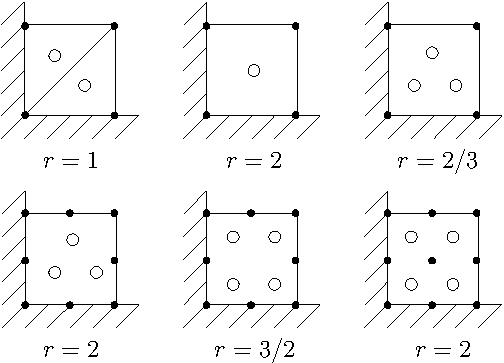
\includegraphics{dis-p-el}
\end{center}
\end{frame}


% ==============================================================================
% SECTION 4: Integración Selectiva
% ==============================================================================
%%%%%%%%%%%%%%%%%%%%%%%%%%%%%%%%%%%%%%%%%%%%%%%%%%%%%%%%%%%%%%%%%%%%%%%%%%
\section[Integración]{Integración selectiva}
%%%%%%%%%%%%%%%%%%%%%%%%%%%%%%%%%%%%%%%%%%%%%%%%%%%%%%%%%%%%%%%%%%%%%%%%%%
\begin{frame}{Integración selectiva y reducida}
  \begin{uicard}[title=Descomposición de la matriz de rigidez elemental $K^e$, top=3pt, bottom=4pt, left=8pt, right=8pt, attach title to upper={\par\vspace{0.08cm}}]
    \small
    $$K^e = \int_{\Omega_e} B^T D B \, d\Omega = \underbrace{\int_{\Omega_e} B^T D_{\lambda} B \, d\Omega}_{K_{\text{vol}}^e \text{ (Volumétrica)}} + \underbrace{\int_{\Omega_e} B^T D_{\mu} B \, d\Omega}_{K_{\text{dev}}^e \text{ (Desviadora)}}$$
  \end{uicard}

  \vspace{0.15cm}

  \begin{uicard}[title=Regla de integración Gaussiana, top=3pt, bottom=4pt, left=8pt, right=8pt, attach title to upper={\par\vspace{0.08cm}}]
    \small
    \begin{itemize}
      \item \textbf{Integración completa ($2 \times 2$ Gauss):} Se aplica a la parte desviadora $K_{\text{dev}}^e$. Evita modos espúreos.
      \item \textbf{Integración reducida ($1 \times 1$ Gauss):} Se aplica a la parte volumétrica $K_{\text{vol}}^e$. Relaja las restricciones y elimina el bloqueo.
    \end{itemize}
    \par\vspace{0.05cm}
    \centering
    \textcolor{TextDark!70}{\footnotesize \textbf{Teorema de Malkus-Hughes:} Demuestra la equivalencia entre integración selectiva y formulaciones mixtas.}
  \end{uicard}
\end{frame}
% ==============================================================================
% SECTION 5: Hourglass
% ==============================================================================
%%%%%%%%%%%%%%%%%%%%%%%%%%%%%%%%%%%%%%%%%%%%%%%%%%%%%%%%%%%%%%%%%%%%%%%%%%
\section[Hourglass]{Control de Hourglass}
%%%%%%%%%%%%%%%%%%%%%%%%%%%%%%%%%%%%%%%%%%%%%%%%%%%%%%%%%%%%%%%%%%%%%%%%%%
\begin{frame}{Control de Hourglass}
  \begin{uicard}[title=Origen del problema, top=2pt, bottom=3pt, left=6pt, right=6pt, attach title to upper={\par\vspace{0.05cm}}]
    \small
\begin{itemize}
      \item \textbf{Geometría de la flexión:} En un elemento flectado, las extensiones y compresiones máximas ocurren en los bordes, mientras que el centro ($\xi=0, \eta=0$) permanece en la \textbf{fibra neutra}.
      \item \textbf{1 único punto de Gauss:} el algoritmo evalúa la deformación justo donde la flexión vale cero.
      \item \textbf{Consecuencia:} flectar el elemento no cuesta energía ($\lambda_{\text{flex}} = 0$), permitiendo mallas que se deforman sin resistencia (\emph{hourglassing}).
    \end{itemize}
  \end{uicard}

  \vspace{0.01cm}

  \begin{uicard}[title=Estrategia de estabilización, top=2pt, bottom=3pt, left=6pt, right=6pt, attach title to upper={\par\vspace{0.05cm}}]
    \small
    \begin{itemize}
      \item Se añade una rigidez artificial $K_h$ a la $K^e$:
        $$K^e = K_{1\times 1} + K_h$$
      \item Se diseña $K_h$ mediante un vector de estabilización de Flanaggan-Belytschko para penalizar \textbf{únicamente} los modos de \emph{hourglass} sin rigidizar otros modos.
    \end{itemize}
  \end{uicard}
\end{frame}

% ==============================================================================
% SECTION 6: B-BAR
% ==============================================================================
%%%%%%%%%%%%%%%%%%%%%%%%%%%%%%%%%%%%%%%%%%%%%%%%%%%%%%%%%%%%%%%%%%%%%%%%%%
\section[B-Bar]{Formulacion B-bar}
%%%%%%%%%%%%%%%%%%%%%%%%%%%%%%%%%%%%%%%%%%%%%%%%%%%%%%%%%%%%%%%%%%%%%%%%%%
\begin{frame}{La formulación $\overline{\bm{B}}$}
  \begin{uicard}[title=Descomposición aditiva de la matriz $\bm{B}$, top=2pt, bottom=3pt, left=6pt, right=6pt, attach title to upper={\par\vspace{0.05cm}}]
    \small
    Definimos el campo de deformaciones como $\bm{\varepsilon} = \overline{\bm{B}} \bm{d}$, con $\bm{B} = (\bm{B}^1, \bm{B}^2, \bm{B}^3, \bm{B}^4)$ y:
    $$\bm{B}^A = \begin{pmatrix} N_{,1}^A & 0 \\ 0 & N_{,2}^A \\ N_{,2}^A & N_{,1}^A \end{pmatrix}$$
  \end{uicard}

  \vspace{0.05cm}

  \begin{uicard}[title=Separación volumétrica-desviadora y evaluación, top=2pt, bottom=3pt, left=6pt, right=6pt, attach title to upper={\par\vspace{0.05cm}}]
    \small
    Descomponemos $\bm{B} = \bm{B}_{\text{vol}} + \bm{B}_{\text{dev}}$, donde la componente volumétrica es:
    $$\bm{B}_{\text{vol}}^A = \frac{1}{3} \begin{pmatrix} N_{,1}^A & N_{,2}^A \\ N_{,1}^A & N_{,2}^A \\ 0 & 0 \end{pmatrix} \qquad \text{y} \qquad \bm{B}_{\text{dev}} = \bm{B} - \bm{B}_{\text{vol}}$$

    Evaluando únicamente la parte volumétrica en el centro isoparamétrico:
    $$\overline{\bm{B}} = \left. \bm{B}_{\text{vol}} \right|_{\bm{\xi}=\bm{0}} + \bm{B}_{\text{dev}}$$
  \end{uicard}
\end{frame}

% ==============================================================================
% SECTION 7: Modos Incompatibles
% ==============================================================================
%%%%%%%%%%%%%%%%%%%%%%%%%%%%%%%%%%%%%%%%%%%%%%%%%%%%%%%%%%%%%%%%%%%%%%%%%%
\section[Incompatibles]{Modos incompatibles}
%%%%%%%%%%%%%%%%%%%%%%%%%%%%%%%%%%%%%%%%%%%%%%%%%%%%%%%%%%%%%%%%%%%%%%%%%%
\begin{frame}
\frametitle{El método de los modos incompatibles}
\begin{itemize}
\item Concepto: añadir modos de flexión de orden cuadrático.
\item Interpolación del campo de desplazamientos:
$$\bm{u}=\sum_{A=1}^{4} N_{A}(\bm{\xi}) \bm{d}_{A}+\sum_{I=1}^{2}
\tilde{N}_{I}(\bm{\xi}) \bm{\alpha}_{I}$$
\begin{xalignat*}{3}
\textrm{siendo:} & \mbox{} &
\tilde{N}_{1}(\bm{\xi})&=\frac{1}{2}(\xi^2-1), &
\tilde{N}_{2}(\bm{\xi})&=\frac{1}{2}(\eta^2-1)
\end{xalignat*}
\item Los $\bm{\alpha}_{I}$ son grados de libertad internos a nivel de cada
elemento.
\item Deformaciones: $\bm{\varepsilon}=\bm{B} \bm{d} + \bm{G} \bm{\alpha}$
$$
\bm{G}=\left[ \bm{G}_{1} \; \bm{G}_{2} \right] 
\;\;\;\;\;\;
\bm{G}_{I}=
\left(
\begin{array}{cc}
\tilde{N}_{I,1}&0 \\
0& \tilde{N}_{I,2}\\
\tilde{N}_{I,2}&\tilde{N}_{I,1}
\end{array}
\right)
$$
\end{itemize}
\end{frame}

% ==============================================================================
% SECTION 8: Deformaciones supuestas
% ==============================================================================
%%%%%%%%%%%%%%%%%%%%%%%%%%%%%%%%%%%%%%%%%%%%%%%%%%%%%%%%%%%%%%%%%%%%%%%%%%
\section[E.A.S.]{Deformaciones supuestas}
%%%%%%%%%%%%%%%%%%%%%%%%%%%%%%%%%%%%%%%%%%%%%%%%%%%%%%%%%%%%%%%%%%%%%%%%%%%%%%
\begin{frame}{Formulación E.A.S.}{Enhanced Assumed Strain (Simo-Rifai)}
  \begin{uicard}[title=Concepto variacional, top=2pt, bottom=3pt, left=6pt, right=6pt, attach title to upper={\par\vspace{0.05cm}}]
    \small
    Mejoramos el campo de deformaciones compatibles $\bm{\nabla}^{\text{S}}\bm{u}$ mediante un campo de deformaciones ``mejoradas0'' independientes $\tilde{\bm{\varepsilon}}$:
    $$\bm{\varepsilon} = \bm{\nabla}^{\text{S}}\bm{u} + \tilde{\bm{\varepsilon}}$$
  \end{uicard}

  \vspace{0.05cm}

  \begin{uicard}[title=Ventajas de la formulación E.A.S., top=2pt, bottom=3pt, left=6pt, right=6pt, attach title to upper={\par\vspace{0.05cm}}]
    \small
    \begin{itemize}
      \item \textbf{Consistencia variacional:} Basado en un principio multifase (Hu-Washizu modificado).
      \item \textbf{Generalización:} Resuelve las deficiencias de Wilson-Taylor en elementos distorsionados y permite extensión a no linealidad geométrica.
      \item \textbf{Pasa el Patch Test:} Garantiza la convergencia de forma rigurosa.
    \end{itemize}
  \end{uicard}
\end{frame}
%%%%%%%%%%%%%%%%%%%%%%%%%%%%%%%%%%%%%%%%%%%%%%%%%%%%%%%%%%%%%%%%%%%%%%%%%%
\begin{frame}
\frametitle{Diseño de elementos: Metodología}
\begin{enumerate}
\item Definir en el espacio isoparamétrico una matriz de interpolación 
${\bf E}({\bm \xi})$, tal que el campo de deformaciones mejoradas tenga 
la expresión:
$$
{\tilde {\bf E}}({\bm \xi})={\bf E}({\bm \xi})\cdot {\bm \alpha}^{e}
\qquad {\bm \alpha}^{e} \in {\cal R}^{n_{\varepsilon}}
$$
\item Obtener la expresión de la matriz ${\bf G}({\bm \xi})$ de interpolación
del campo de deformaciones mejoradas en el espacio físico
${\tilde {\bm \varepsilon}}({\bm \xi})$
$$
{\bf G}({\bm \xi})=\frac{j_{0}}{j({\bm \xi})}{\bf F}_{0}^{-{\rm T}}
{\bf E}({\bf \xi}) 
$$
\end{enumerate}
\end{frame}
%%%%%%%%%%%%%%%%%%%%%%%%%%%%%%%%%%%%%%%%%%%%%%%%%%%%%%%%%%%%%%%%%%%%%%%%%%
\begin{frame}
\frametitle{Diseño de elementos: Ejemplos}
\begin{footnotesize}
\begin{itemize}
\item Elemento Q4/E4 (Wilson-Taylor)
$$
{\bm E}({\bm \xi})=
\left(
\begin{array}{cccc}
\xi&0&0&0 \\
0  &\eta&0&0\\
0  &   0&\xi&\eta
\end{array}
\right)
$$
\item Elemento Q4/E5 (Simo-Rifai)
$$
{\bm E}({\bm \xi})=
\left(
\begin{array}{ccccc}
\xi&0&0&0&\xi \eta \\
0  &\eta&0&0&-\xi \eta \\
0  &   0&\xi&\eta&\xi^2-\eta^2
\end{array}
\right)
$$
\item Elemento Q4/E7 (Andelfinger-Ramm)
$$
{\bm E}({\bm \xi})=
\left(
\begin{array}{ccccccc}
\xi&0&0&0&\xi \eta&0&0 \\
0  &\eta&0&0&0&\xi \eta&0\\
0  &   0&\xi&\eta&0&0&\xi \eta
\end{array}
\right)
$$
\end{itemize}
\end{footnotesize}
\end{frame}


% ==============================================================================
% SECTION 9: Conclusiones
% ==============================================================================
%%%%%%%%%%%%%%%%%%%%%%%%%%%%%%%%%%%%%%%%%%%%%%%%%%%%%%%%%%%%%%%%%%%%%%%%%%
\section[Conclusiones]{Conclusiones}
%%%%%%%%%%%%%%%%%%%%%%%%%%%%%%%%%%%%%%%%%%%%%%%%%%%%%%%%%%%%%%%%%%%%%%%%%%%%%%
\begin{frame}{Comparativa de tecnologías}
\begin{uicard}[title=Resumen de rigideces frente a flexión ($\lambda_{\text{BG}}$), top=2pt, bottom=3pt, left=6pt, right=6pt, attach title to upper={\par\vspace{0.05cm}}]
    \scriptsize
    \centering
    \renewcommand{\arraystretch}{1.8} % Aumenta la altura vertical de cada fila
    \begin{tabular}{||c|c|c||}
      \hline \hline
      Elemento & Modo $\lambda_{\text{BG1}}$ & Modo $\lambda_{\text{BG2}}$ \\ \hline \hline
      $Q4$ (estándar) & $(\mu + (\lambda+2\mu)r^2)/3r$ & $(\mu r^2 + \lambda+2\mu)/3r$ \\ \hline
      $Q4R$ (int. reducida) & $0$ & $0$ \\ \hline
      $\overline{\bm{B}}$ & $(9\mu + r^2(\lambda+10\mu))/27r$ & $(9r^2\mu + (\lambda+10\mu))/27r$ \\ \hline
      $Q1/E4$ (EAS / Incompat.) & $\frac{4r\mu(\lambda+\mu)}{3(\lambda+2\mu)}$ & $\frac{4\mu(\lambda+\mu)}{3r(\lambda+2\mu)}$ \\
      \hline \hline
    \end{tabular}
  \end{uicard}

  \vspace{0.05cm}

  \begin{uicard}[title=Diagnóstico final de rendimiento, top=2pt, bottom=3pt, left=6pt, right=6pt, attach title to upper={\par\vspace{0.05cm}}]
    \footnotesize
    \begin{itemize}
      \item \textbf{$Q4$ y $\overline{\bm{B}}$:} Se bloquean en flexión de elementos esbeltos ($r \to \infty \Rightarrow \lambda_{\text{BG}} \to \infty$).
      \item \textbf{$Q4R$:} Elimina el bloqueo pero tiene energía nula ($\lambda_{\text{BG}} = 0 \Rightarrow$ \emph{hourglassing}).
      \item \textbf{$Q1/E4$:} En el límite incompresible ($\lambda \to \infty$), $\lambda_{\text{BG}} \to \frac{4\mu}{3} < \infty$. \\
      \textbf{\textcolor{Turquoise}{¡Cero bloqueo!}}
    \end{itemize}
  \end{uicard}
\end{frame}
%%%%%%%%%%%%%%%%%%%%%%%%%%%%%%%%%%%%%%%%%%%%%%%%%%%%%%%%%%%%%%%%%%%%%%%%%%%%%%
\begin{frame}
\frametitle{Ejemplos. Sensibilidad a la distorsión}

\begin{center}
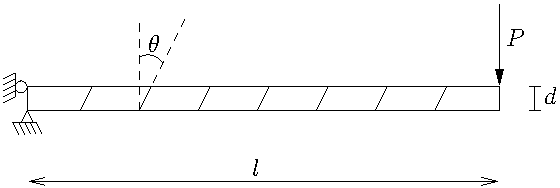
\includegraphics{mens-sim}

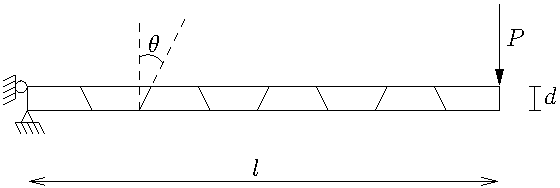
\includegraphics{mens-asim}
\end{center}
\end{frame}
%%%%%%%%%%%%%%%%%%%%%%%%%%%%%%%%%%%%%%%%%%%%%%%%%%%%%%%%%%%%%%%%%%%%%%%%%%%%%%
\begin{frame}
\frametitle{Ejemplos. Sensibilidad a la distorsión}
\begin{small}
\begin{center}
\begin{tabular}{||c|c|c|c||}
\hline \hline
$\theta    $& $Q4$        &$\overline{B}$& $Q1/E4$   \\ \hline \hline
$0^{\circ} $&$0.12458$    &$0.12995$     &$0.99664$  \\ \hline
$15^{\circ}$&$0.11080$    &$0.11935$     &$0.96783$  \\ \hline
$30^{\circ}$&$0.08022$    &$0.09275$     &$0.91632$  \\ \hline
$45^{\circ}$&$0.04985$    &$0.06101$     &$0.88451$  \\ \hline
\end{tabular}
\end{center}

\begin{center}
\begin{tabular}{||c|c|c|c|c|c||}
\hline \hline
$\theta$& $Q4$       &$\overline{B}$&$Q1/E4$ &$Q1/E5$
&$Q1/E7$ \\ \hline \hline
$ 0^{\circ}$ & $0.12458$  &$0.12995$
&$0.99664$&$0.99664$&$0.99664$ \\ \hline
$15^{\circ}$ & $0.09959$  &$0.10467$
&$0.45105$&$0.45107$&$0.45107$ \\ \hline
$30^{\circ}$ & $0.06148$  &$0.06563$
&$0.26135$&$0.26143$&$0.26145$ \\ \hline
$45^{\circ}$ & $0.03627$  &$0.03906$
&$0.19824$&$0.19845$&$0.19849$ \\ \hline
\end{tabular}
\end{center}
\end{small}
\end{frame}
%%%%%%%%%%%%%%%%%%%%%%%%%%%%%%%%%%%%%%%%%%%%%%%%%%%%%%%%%%%%%%%%%%%%%%%%%%%%%%
\begin{frame}
\frametitle{Ejemplos. Ensayo de identación de Prandtl}
\begin{center}
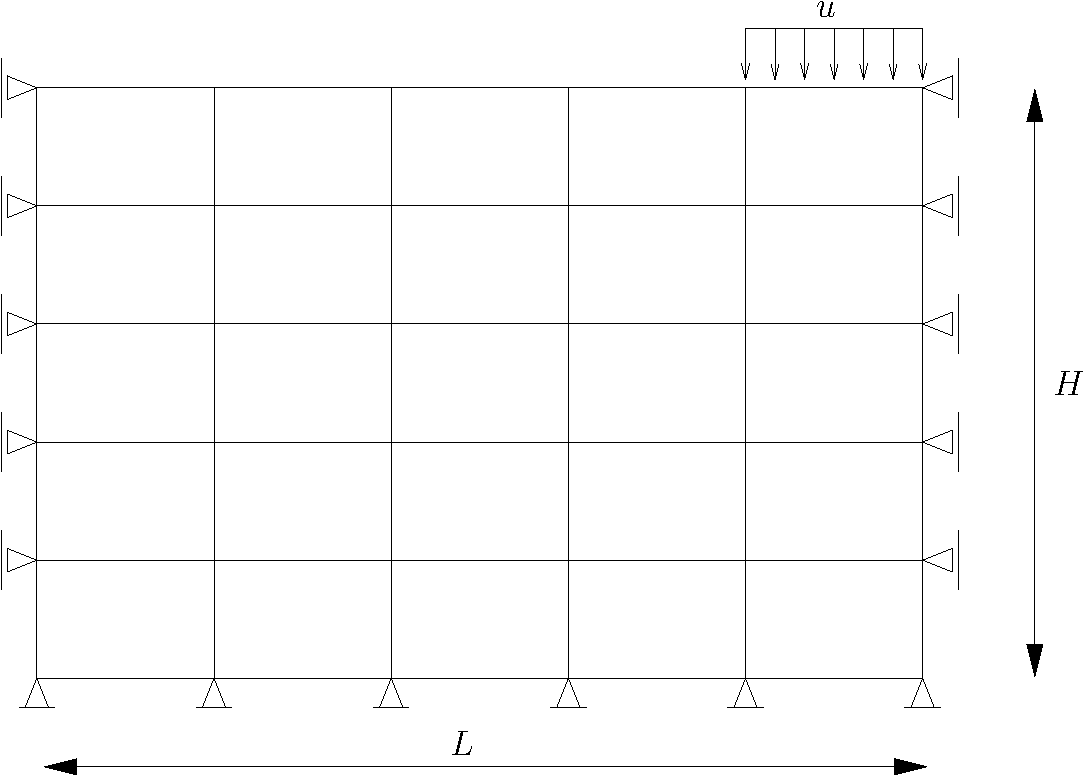
\includegraphics[width=\textwidth]{punch}
\end{center}
\end{frame}
%%%%%%%%%%%%%%%%%%%%%%%%%%%%%%%%%%%%%%%%%%%%%%%%%%%%%%%%%%%%%%%%%%%%%%%%%%%%%%
\begin{frame}
\frametitle{Ejemplos. Ensayo de identación de Prandtl}
\begin{center}
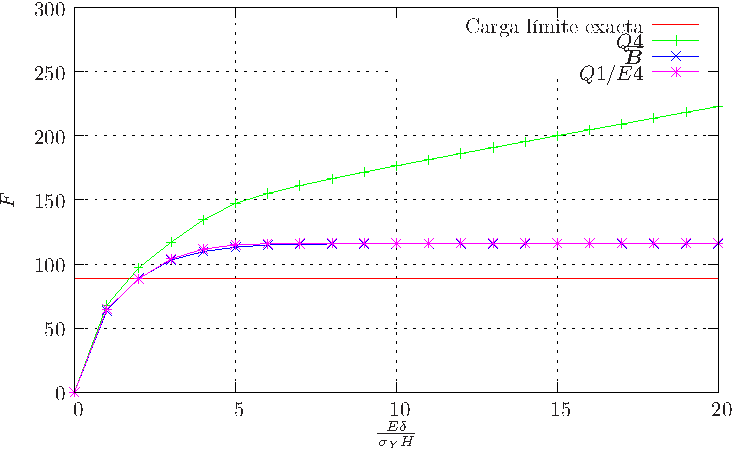
\includegraphics[width=\textwidth]{punchfd}
\end{center}
\end{frame}
%%%%%%%%%%%%%%%%%%%%%%%%%%%%%%%%%%%%%%%%%%%%%%%%%%%%%%%%%%%%%%%%%%%%%%%%%%%%%%
\begin{frame}
\frametitle{Ejemplos. La membrana de Cook}

\vspace{1cm}
\begin{center}
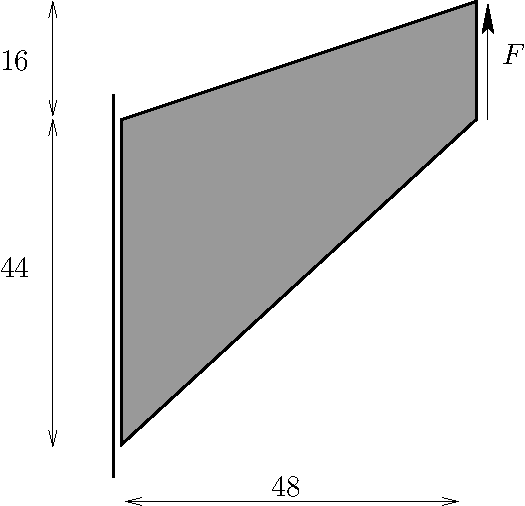
\includegraphics[width=0.65\textwidth]{cook}
\end{center}
\end{frame}
%%%%%%%%%%%%%%%%%%%%%%%%%%%%%%%%%%%%%%%%%%%%%%%%%%%%%%%%%%%%%%%%%%%%%%%%%%%%%%
\begin{frame}
\frametitle{Ejemplos. La membrana de Cook}

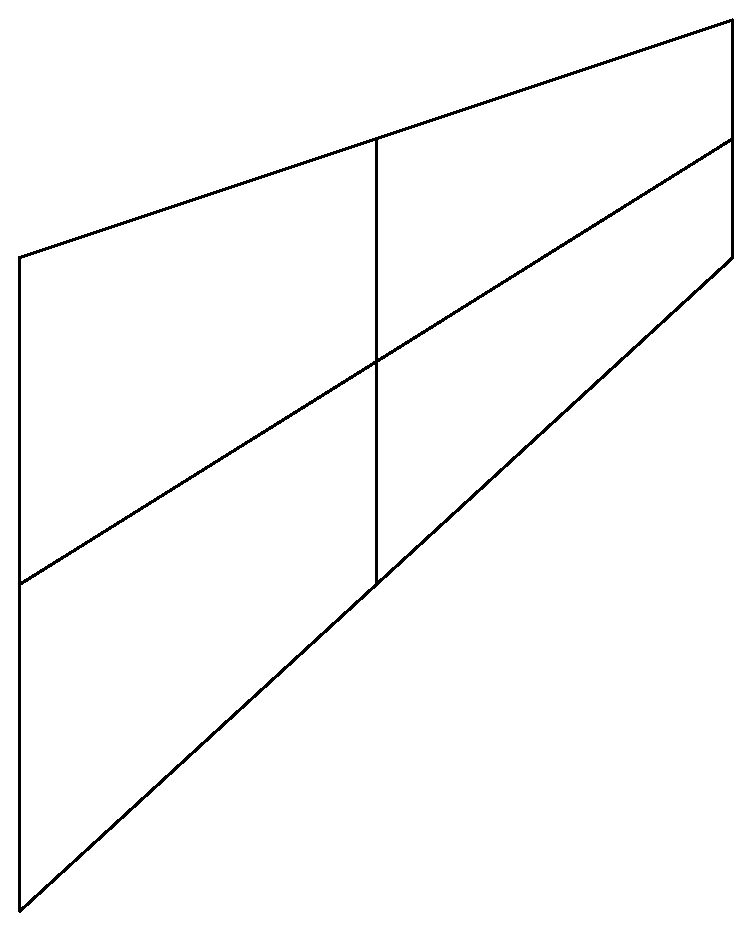
\includegraphics[width=20mm]{cook2}
\hfill
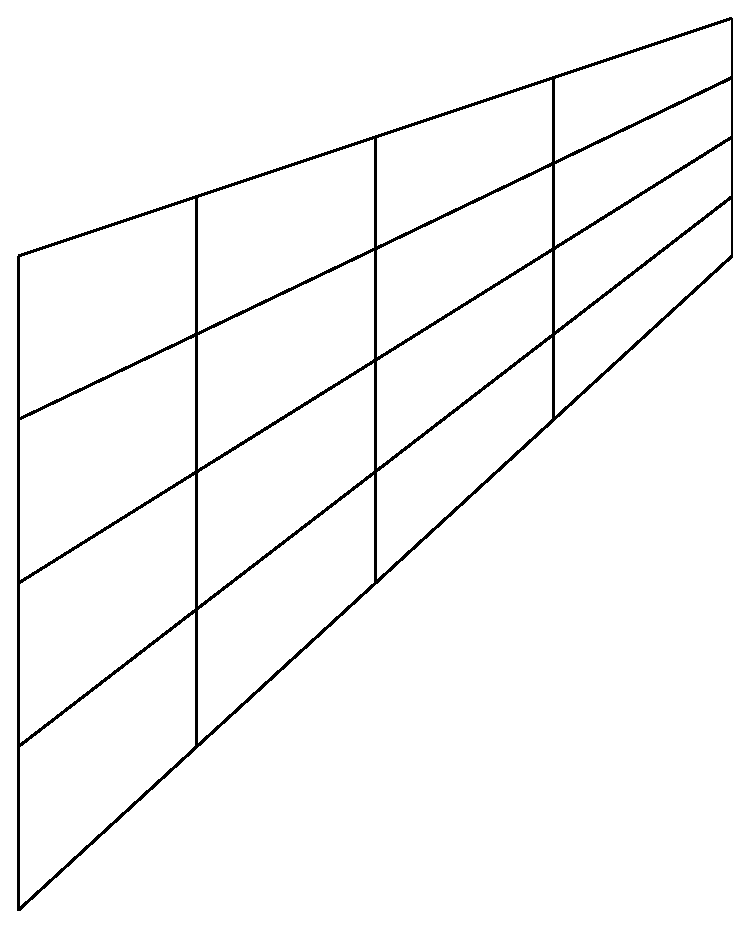
\includegraphics[width=20mm]{cook4}
\hfill
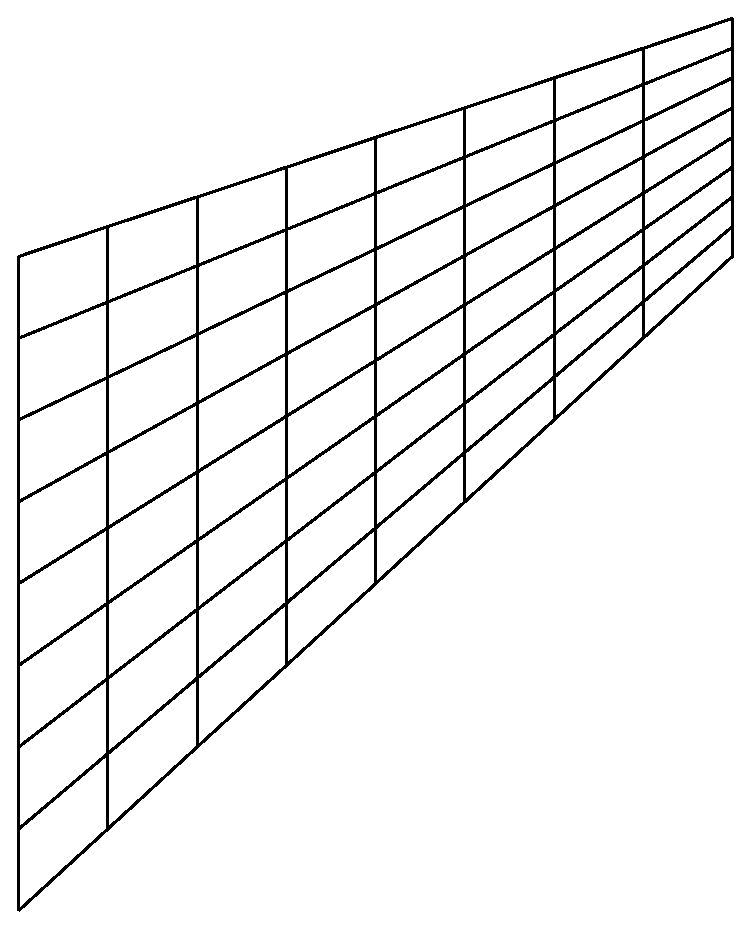
\includegraphics[width=20mm]{cook8}

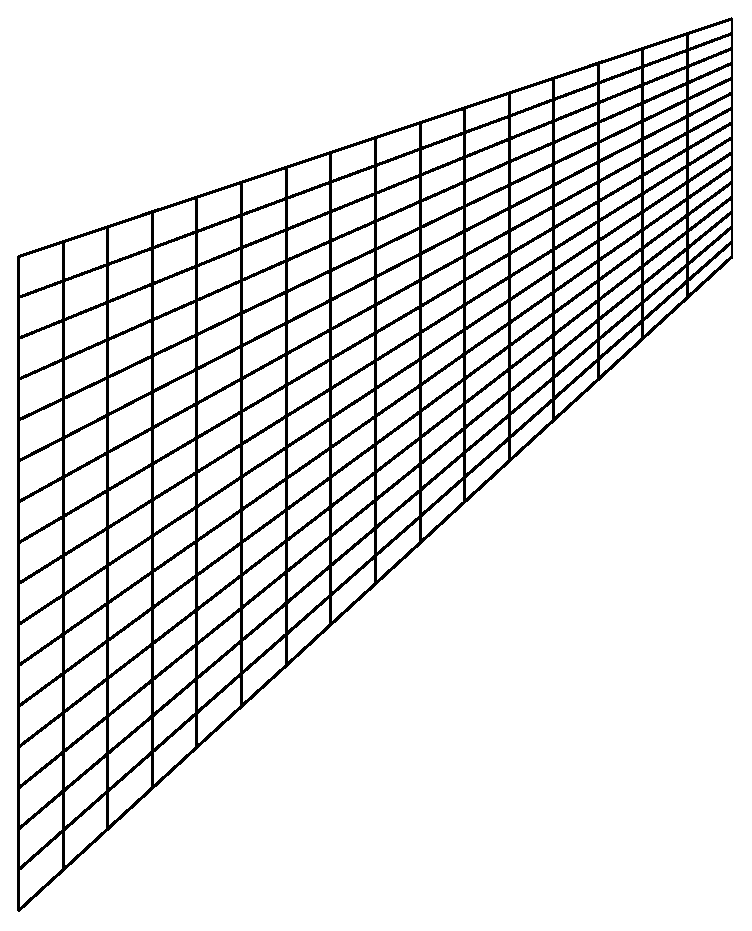
\includegraphics[width=20mm]{cook16}
\hfill
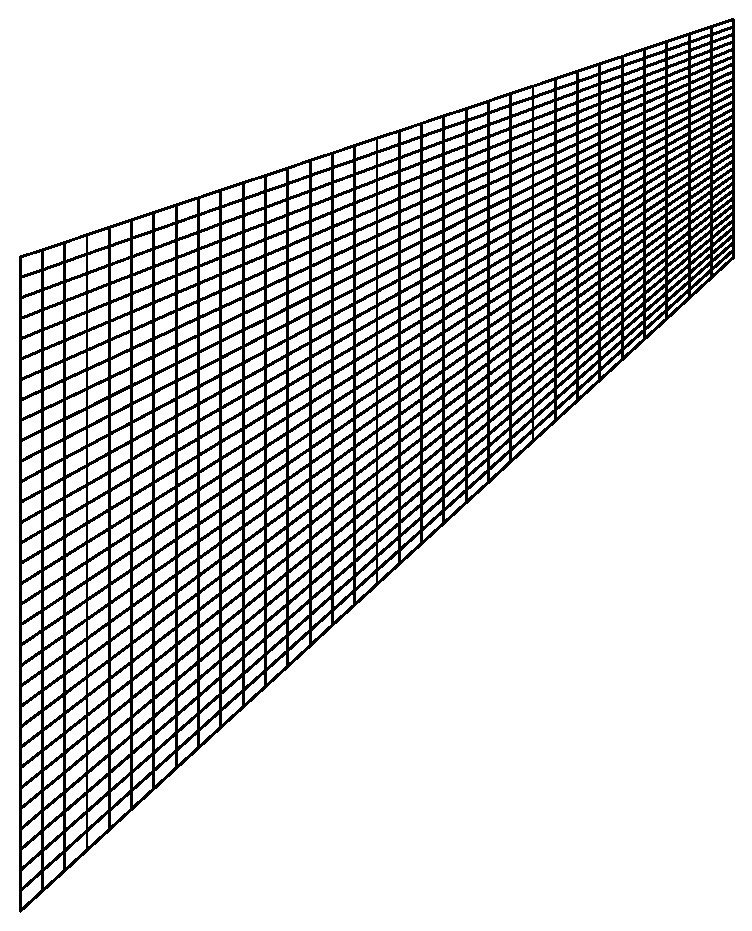
\includegraphics[width=20mm]{cook32}
\hfill
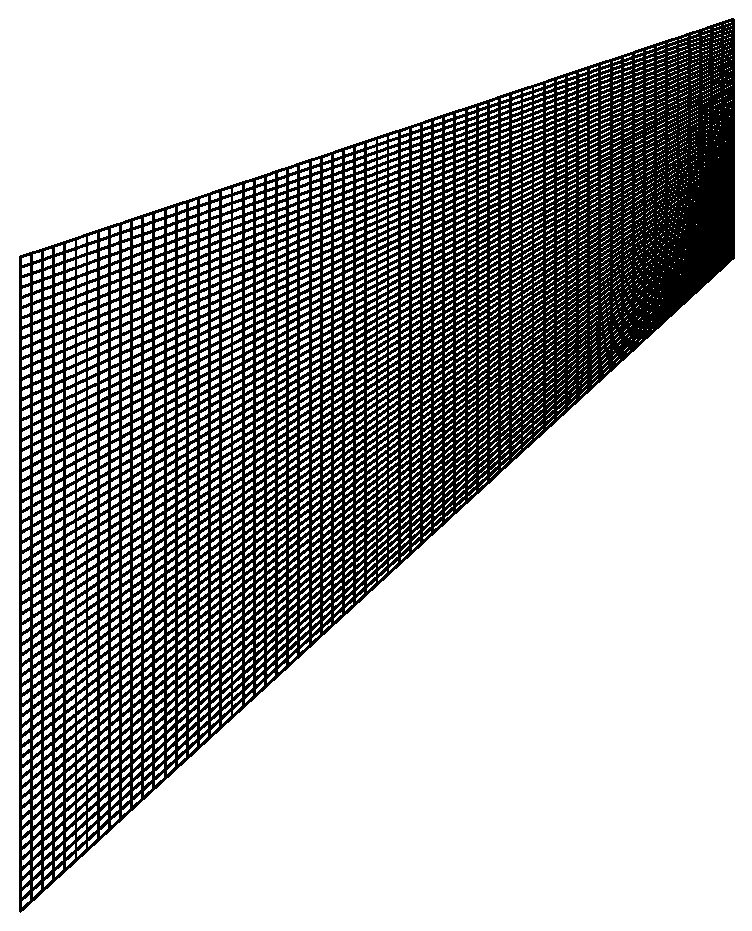
\includegraphics[width=20mm]{cook64}
\end{frame}
%%%%%%%%%%%%%%%%%%%%%%%%%%%%%%%%%%%%%%%%%%%%%%%%%%%%%%%%%%%%%%%%%%%%%%%%%%%%%%
\begin{frame}

\frametitle{Ejemplos. La membrana de Cook}
\begin{center}
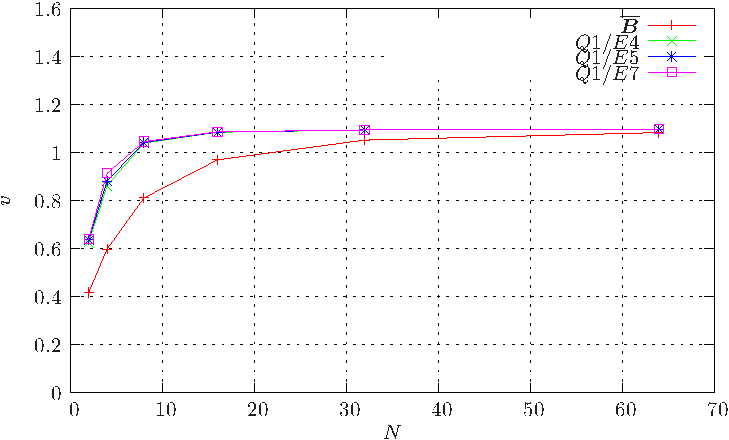
\includegraphics[width=\textwidth]{cookcon}
\end{center}
\begin{align}
v &:\textrm{ Flecha} \nonumber \\
N &:\textrm{ Elementos por lado} \nonumber
\end{align}
\end{frame}
%%%%%%%%%%%%%%%%%%%%%%%%%%%%%%%%%%%%%%%%%%%%%%%%%%%%%%%%%%%%%%%%%%%%%%%%%%


% ==============================================================================
% SECTION Extra: BIBLIOGRAFÍA
% ==============================================================================
\begin{frame}{Para ampliar este tema\dots}{}
  \begin{thebibliography}{10}
    \bibitem{Hughes}
    \textbf{HUGHES, T.J.R.}
    \newblock \emph{The Finite Element Method. Linear Static and Dynamic Finite Element Analysis.}
    \newblock Dover Publications Inc., 2000.
    \vspace{0.4cm}
    
    \bibitem{Onate}
    \textbf{OÑATE, E.}
    \newblock \emph{Cálculo de Estructuras por el Método de Elementos Finitos. Análisis estático lineal.}
    \newblock CIMNE. Segunda edición, 1995.
    \vspace{0.4cm}
    
    \bibitem{Felippa}
    \textbf{FELIPPA, C.A.}
    \newblock \emph{Introduction to Finite Element Methods (ASEN 5007).}
    \newblock University of Colorado at Boulder.
  \end{thebibliography}
\end{frame}

% ==============================================================================
% AGRADECIMIENTOS
% ==============================================================================
\begin{frame}{Reconocimiento y Agradecimiento}{}
  \vfill
  \begin{uicard}[borderline north={4pt}{0pt}{Turquoise}, left=15pt, right=15pt, top=18pt, bottom=18pt]
    \centering
    {\normalsize \textcolor{TextDark}{
      Nuestro sincero agradecimiento al \textbf{Profesor D. Felipe Gabaldón Castillo} por su dedicación a esta asignatura a lo largo de los años y por su generosidad al ceder todo el material docente y bibliográfico que sirve de base para estas lecciones.
    }}\\[0.6cm]
    
    \textcolor{Turquoise}{\small\bfseries Dpto. de Mecánica de Medios Continuos y Teoría de Estructuras}
  \end{uicard}
  \vfill
\end{frame}

\end{document}